\documentclass[11pt,]{article}
\usepackage[left=1in,top=1in,right=1in,bottom=1in]{geometry}
\newcommand*{\authorfont}{\fontfamily{phv}\selectfont}
  \usepackage[]{mathpazo}
  
  
  \usepackage[T1]{fontenc}
\usepackage[utf8]{inputenc}



\usepackage{abstract}
\renewcommand{\abstractname}{}    % clear the title
\renewcommand{\absnamepos}{empty} % originally center

\renewenvironment{abstract}
{{%
  \setlength{\leftmargin}{0mm}
  \setlength{\rightmargin}{\leftmargin}%
}%
  \relax}
{\endlist}

\makeatletter
\def\@maketitle{%
  \newpage
  %  \null
  %  \vskip 2em%
    %  \begin{center}%
    \let \footnote \thanks
  {\fontsize{18}{20}\selectfont\raggedright  \setlength{\parindent}{0pt} \@title \par}%
}
%\fi
\makeatother


  
  
  \setcounter{secnumdepth}{0}

      \usepackage{color}
  \usepackage{fancyvrb}
  \newcommand{\VerbBar}{|}
  \newcommand{\VERB}{\Verb[commandchars=\\\{\}]}
  \DefineVerbatimEnvironment{Highlighting}{Verbatim}{commandchars=\\\{\}}
  % Add ',fontsize=\small' for more characters per line
  \usepackage{framed}
  \definecolor{shadecolor}{RGB}{248,248,248}
  \newenvironment{Shaded}{\begin{snugshade}}{\end{snugshade}}
  \newcommand{\KeywordTok}[1]{\textcolor[rgb]{0.13,0.29,0.53}{\textbf{#1}}}
  \newcommand{\DataTypeTok}[1]{\textcolor[rgb]{0.13,0.29,0.53}{#1}}
  \newcommand{\DecValTok}[1]{\textcolor[rgb]{0.00,0.00,0.81}{#1}}
  \newcommand{\BaseNTok}[1]{\textcolor[rgb]{0.00,0.00,0.81}{#1}}
  \newcommand{\FloatTok}[1]{\textcolor[rgb]{0.00,0.00,0.81}{#1}}
  \newcommand{\ConstantTok}[1]{\textcolor[rgb]{0.00,0.00,0.00}{#1}}
  \newcommand{\CharTok}[1]{\textcolor[rgb]{0.31,0.60,0.02}{#1}}
  \newcommand{\SpecialCharTok}[1]{\textcolor[rgb]{0.00,0.00,0.00}{#1}}
  \newcommand{\StringTok}[1]{\textcolor[rgb]{0.31,0.60,0.02}{#1}}
  \newcommand{\VerbatimStringTok}[1]{\textcolor[rgb]{0.31,0.60,0.02}{#1}}
  \newcommand{\SpecialStringTok}[1]{\textcolor[rgb]{0.31,0.60,0.02}{#1}}
  \newcommand{\ImportTok}[1]{#1}
  \newcommand{\CommentTok}[1]{\textcolor[rgb]{0.56,0.35,0.01}{\textit{#1}}}
  \newcommand{\DocumentationTok}[1]{\textcolor[rgb]{0.56,0.35,0.01}{\textbf{\textit{#1}}}}
  \newcommand{\AnnotationTok}[1]{\textcolor[rgb]{0.56,0.35,0.01}{\textbf{\textit{#1}}}}
  \newcommand{\CommentVarTok}[1]{\textcolor[rgb]{0.56,0.35,0.01}{\textbf{\textit{#1}}}}
  \newcommand{\OtherTok}[1]{\textcolor[rgb]{0.56,0.35,0.01}{#1}}
  \newcommand{\FunctionTok}[1]{\textcolor[rgb]{0.00,0.00,0.00}{#1}}
  \newcommand{\VariableTok}[1]{\textcolor[rgb]{0.00,0.00,0.00}{#1}}
  \newcommand{\ControlFlowTok}[1]{\textcolor[rgb]{0.13,0.29,0.53}{\textbf{#1}}}
  \newcommand{\OperatorTok}[1]{\textcolor[rgb]{0.81,0.36,0.00}{\textbf{#1}}}
  \newcommand{\BuiltInTok}[1]{#1}
  \newcommand{\ExtensionTok}[1]{#1}
  \newcommand{\PreprocessorTok}[1]{\textcolor[rgb]{0.56,0.35,0.01}{\textit{#1}}}
  \newcommand{\AttributeTok}[1]{\textcolor[rgb]{0.77,0.63,0.00}{#1}}
  \newcommand{\RegionMarkerTok}[1]{#1}
  \newcommand{\InformationTok}[1]{\textcolor[rgb]{0.56,0.35,0.01}{\textbf{\textit{#1}}}}
  \newcommand{\WarningTok}[1]{\textcolor[rgb]{0.56,0.35,0.01}{\textbf{\textit{#1}}}}
  \newcommand{\AlertTok}[1]{\textcolor[rgb]{0.94,0.16,0.16}{#1}}
  \newcommand{\ErrorTok}[1]{\textcolor[rgb]{0.64,0.00,0.00}{\textbf{#1}}}
  \newcommand{\NormalTok}[1]{#1}
        
    
    \title{ST790: Quantopian Final Project  }
  
  
  
  \author{}
  
  
  \date{}

\usepackage{titlesec}

\titleformat*{\section}{\normalsize\bfseries}
\titleformat*{\subsection}{\normalsize\itshape}
\titleformat*{\subsubsection}{\normalsize\itshape}
\titleformat*{\paragraph}{\normalsize\itshape}
\titleformat*{\subparagraph}{\normalsize\itshape}


  
      
  
  \newtheorem{hypothesis}{Hypothesis}
\usepackage{setspace}

\makeatletter
\@ifpackageloaded{hyperref}{}{%
  \ifxetex
  \PassOptionsToPackage{hyphens}{url}\usepackage[setpagesize=false, % page size defined by xetex
                                                 unicode=false, % unicode breaks when used with xetex
                                                 xetex]{hyperref}
  \else
    \PassOptionsToPackage{hyphens}{url}\usepackage[unicode=true]{hyperref}
  \fi
}

\@ifpackageloaded{color}{
  \PassOptionsToPackage{usenames,dvipsnames}{color}
}{%
  \usepackage[usenames,dvipsnames]{color}
}
\makeatother
\hypersetup{breaklinks=true,
bookmarks=true,
pdfauthor={},
pdfkeywords = {},  
pdftitle={ST790: Quantopian Final Project},
colorlinks=true,
citecolor=blue,
urlcolor=blue,
linkcolor=magenta,
pdfborder={0 0 0}}
\urlstyle{same}  % don't use monospace font for urls

% set default figure placement to htbp
\makeatletter
\def\fps@figure{htbp}
\makeatother

\setlength{\abovedisplayskip}{.2pt}
\setlength{\belowdisplayskip}{.2pt}
\usepackage{placeins}
\usepackage{setspace}
\usepackage{chngcntr}
\usepackage{multicol}
\usepackage{lscape}
\counterwithin{figure}{section}
\counterwithin{table}{section}
\usepackage{mathrsfs}
\usepackage{mathtools}
\usepackage{multirow}
\newtheorem{theorem}{Theorem}
\usepackage[linesnumbered,algoruled,boxed,lined,commentsnumbered]{algorithm2e}
\usepackage{bm}
\newcommand{\blandscape}{\begin{landscape}}
\newcommand{\elandscape}{\end{landscape}}


% add tightlist ----------
\providecommand{\tightlist}{%
\setlength{\itemsep}{0pt}\setlength{\parskip}{0pt}}

\begin{document}

% \pagenumbering{arabic}% resets `page` counter to 1 
%
% \maketitle

{% \usefont{T1}{pnc}{m}{n}
\setlength{\parindent}{0pt}
\thispagestyle{plain}
{\fontsize{18}{20}\selectfont\raggedright 
\maketitle  % title \par  

}

{
  \vskip 13.5pt\relax \normalsize\fontsize{11}{12} 
   
  
}

}






\vskip 6.5pt


\noindent  \section{Introduction}\label{introduction}

As fund managers, we were tasked with constructing a cross-sectional,
long-short US equity strategy on
\href{https://www.quantopian.com/}{Quantopian}. There were not many
explicit constraints on the specific strategy we utilized, but it must
pass the following criteria: (i) trade liquid stocks, (ii) have no more
than 5\% of capital invested in any one asset, (iii) have no more than
10\% net dollar exposure, (iv) achieve mean daily turnover between 5\%
and 65\% over a 63-trading-day rolling window, (v) attain gross leverage
between 0.8x and 1.1x, (vi) have low correlation to the market, (vii)
have less than 20\% exposed to each of the 11 sectors as defined on
Quantopian, and (viii) result in positive returns. While the last return
criteria was not a constraint we included in our optimization, we did
design our algorithm with the rest of the seven criteria in mind.

\section{Trading Strategy}\label{trading-strategy}

The backtests we describe below are derived from the following trading
algorithm:

\begin{enumerate}
\def\labelenumi{\arabic{enumi}.}
\tightlist
\item
  Once a week, we choose a universe of liquid assets from
  \(\texttt{QTradeableStocksUS}\) that pass the following filters:

  \begin{itemize}
  \tightlist
  \item
    It is not trading within 2 days of any earnings announcements as
    assets are generally more volatile within these dates.
  \item
    It has not been announced as an acquistion target. To further reduce
    any possible volatility, we avoid acquisition targets as they often
    pose huge risk to quant strategies.
  \item
    We are able to calculate a 5 day moving average of the
    bull-minus-bear signal from the \(\texttt{StockTwits}\) API.
  \end{itemize}
\item
  Every day, we build an alpha vector for the universe of liquid assets
  filtered from our step above. The alpha model we use is quite simple:
  we rank the assets by its bull-to-bear intensity, averaged over the
  past 5 days as evaluated from \(\texttt{StockTwits}\), and find a set
  of new portfolio weights that maximizes the sum of each asset's weight
  times this alpha value. Our objective defined in
  \(\texttt{MaximizeAlpha}\) is thus simply a function of this sentiment
  datastream as we believe this ranking is similar to expected returns
  of each asset. As a result, our routine effectively goes long on
  assets with high bullish signal and short on those with a high bearish
  signal.\\
\item
  Once a week, we calculate the portfolio that maximizes the
  alpha-weighted sum of our position sizes, subject to the following
  constraints:

  \begin{itemize}
  \tightlist
  \item
    Our portfolio maintains a gross leverage of, or less than, 1.0x.
  \item
    Our portfolio has no more than 5\% in any single asset.
  \item
    Our portfolio does not pass mean daily turnover of 80\%.
  \end{itemize}
\end{enumerate}

With this simple strategy, we achieve the following leaderboard results
at the end of our one-month trading period from November \(1^{st}\) to
November \(30^{th}\):

\begin{table}[ht]
\small
\centering
\begin{tabular}{rllr}
  \hline
 & Metric & Our Result & Overall \\ 
  \hline
1 & rank & 64 & - \\ 
  2 & name & Gray Fox & - \\ 
  3 & score & 0.502 & 0.36 \\ 
  4 & max\_beta\_to\_spy\_126day & 0.076 & 0.14 \\ 
  5 & max\_cumulative\_common\_returns & 0.009 & 0.04 \\ 
  6 & max\_leverage & 1.047 & 1.05 \\ 
  7 & max\_max\_drawdown & 0 & -0.00 \\ 
  8 & max\_net\_dollar\_exposure & 0.032 & 0.04 \\ 
  9 & max\_total\_returns & 0.025 & 0.14 \\ 
  10 & min\_total\_returns & -0.007 & -0.02 \\ 
  11 & max\_turnover & 0.905 & 1.07 \\ 
  12 & max\_volatility\_126day & 0.044 & 0.06 \\ 
   \hline
\end{tabular}
\end{table}

Key to our strategy is the output from the \texttt{bull\_minus\_bear}
API call as it is this signal that is fed into the optimization function
and this result that determines the order size of each asset. While we
do not have exact clarity on the natural language processing engine that
calculates the bullish intensity and bearish intensity of a stock, we do
know how the \texttt{bull\_minus\_bear} signal arises; traders attached
either a bull emoji or a bear emoji to any message they release on the
\texttt{StockTwits} platform as well as a ticker symbol that identifies
which asset is under discussion. While traders attached a clear label to
the asset of interest, \texttt{StockTwits} also has an in-house
proprietary algorithm that processes some of the language in the message
to ascribe an intensity level of the bull or bear indicator. Messages
across the \texttt{StockTwits} platform is thus aggregated to arrive a
sentiment score that is a function of subtracting the bearish intensity
from the bullish intensity result.

\subsection{Choice of the sentiment
score}\label{choice-of-the-sentiment-score}

In addition to the ease of implementation, we chose to rely on the
sentiment factor as it seems to have some good characteristics, namely:

\begin{enumerate}
\def\labelenumi{\arabic{enumi}.}
\item
  \emph{Predictive alpha} We calculated the mean information coefficient
  using the built-in function in \texttt{alphalens} and found our
  sentiment signal matches the direction of actual asset returns. As
  shown in the top-left of the figure below, we only get the full
  exposure of this factor 5 days after this signal becomes available. In
  fact, prior to 5 trading days, it appears the signal hurts us, in that
  its forecast is negative. Counterintuitively, after we cross 5 trading
  days, it appears our sentiment factor gains more predictive power.
  This is further corroborated in the top-right graph in that returns
  are highest when the signal is delayed by four days. Given this
  characteristic, we may want to build greater exposure to this factor
  since it still benefits us after 10 trading days. We can also leverage
  the positive effects of this factor by increasing our turnover
  constraints as it appears it does not hurt our portfolio to keep in
  there for a longer period of time. Nevertheless, the mean information
  coefficient still lingers around 0, suggesting the forecasting
  benefits provided by our sentiment factor may be no better than the
  results we get from randomly selecting our asset weights.
\item
  \emph{Low exposures} We quantified the exposures via the
  \texttt{perf\_attrib} function in \texttt{pyfolio}. As shown in the
  bottom-left, our sentiment factor appears to have relatively low
  exposures throughout, with most of the returns from volatility risk.
  However, there does appear to be persistent exposure to value and
  short term reversal, in that it is shifted to the left of zero; and
  persistent exposure to size and momentum, in that it is shifted to the
  right of zero. Ideally, we would choose a factor that doesn't display
  this skew, but the skew does not appear too large. We also benefit
  from the fact that the width of each of our box and whisker plots are
  not that wide, so our exposures do not vary much over time. Yet, this
  analysis was conducted only over the available sentiment signal in
  2018, so there may be other extended periods prior to 2018 in which
  our factor over or underperforms. Given what we have here, we may want
  to identify asset classes to include in our portfolio that would
  offset the exposure risks identified above.
\end{enumerate}

Unfortunately, when we examine our exposures through cumulative returns
and volatility, we find that our sentiment factor may not be as strong
as we desired. As shown by the left bar graph (bottom-right), most of
our returns are obtained from exposure to common risk factors, and, as
shown in the right bar graph, are in fact driven by these common risk
factors. Ideally, we would like to strip away the contribution from
these common risk factors as portfolio performance from this exposure
can easily be replicated from ETFs or other easy, cost-effective
methods.

\begin{figure}

{\centering 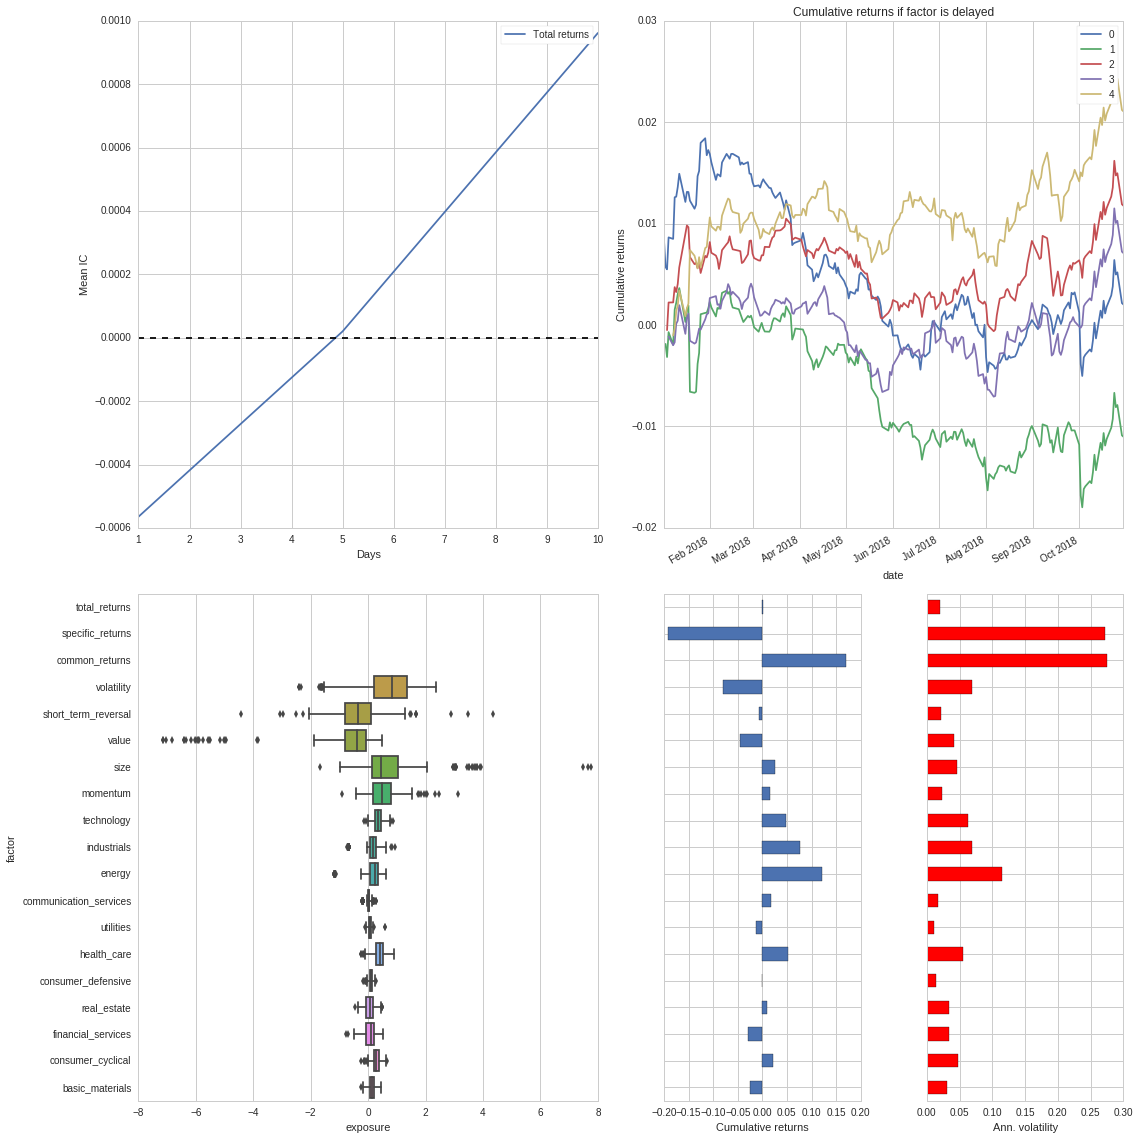
\includegraphics[width=0.8\linewidth]{/home/joyce/workspace/st790-financial-stats/final/download2} 

}

\caption{Examination of (top-right) information coefficient averaged over all possible asset returns, (top-left) cumulative returns when factor is delayed, (bottom-left) risk exposures, and (bottom-right) cumulative returns and volatility.}\label{fig:unnamed-chunk-2}
\end{figure}

\newpage 

\section{Backtesting}\label{backtesting}

Given the extensive literature that sentiment data can predict stock
price, we forged ahead and submitted our trading strategy on Quantopian.
The back test results

\section{Evaluation}\label{evaluation}

\section{Future Improvement}\label{future-improvement}

There are a number of avenues we might consider to improve upon our
simplistic approach:

\begin{enumerate}
\def\labelenumi{\arabic{enumi}.}
\tightlist
\item
  \emph{Using non-trading day sentiment data}: While we relied on what
  was provided to us by \texttt{Stocktwits} we should attempt building
  our own classifier from possiblilty richer sources of messages (e.g.,
  Weibo, Twitter) that can not only provide
\end{enumerate}

\begin{itemize}
\tightlist
\item
  fundamental value measures?
\item
  analyzed bull and bear tagged messages on each asset
\end{itemize}

\section{Sentiment}\label{sentiment}

\begin{itemize}
\item
  looking at relative frequency of words falling under various themes
\item
  SW uses cashtags with stock ticker symbol, like hashtag, to index ppls
  thoughts and ideas about the company and stock
\item
  understand that anything from social media, or anything market or
  finance related comes with its fair share of BS
\item
  stockTwits is no exception
\item
  people ``BuY right now''.. claiming they made excessive gains
\item
\item
  feed stence into algo and know how people are ``feeling''
\item
  rely on a pretty sophistic natural language processing engine can
  parse through online market conversations that can detect trader moods
  bullishness and bearishnes and intensity
\end{itemize}

\subsection{algorithm rules}\label{algorithm-rules}

\section{}\label{section}

\section{Trading Strategy}\label{trading-strategy-1}

\section{November Portfolio
Performance}\label{november-portfolio-performance}

The following displays my portfolio performance between Nov 1 and Nov 30

\section{Back Testing}\label{back-testing}

Shown for three different time periods in the 21st century: - 2000-2002
- 2008-2010 - 2015-2018 \# this doesnt work bc of stocktwits limitation

since we rely on pyschsignal.stocktwits 2007-01-01 to 2018-10-30

\section{Discussion}\label{discussion}

returns, positions, leverage, risk, control

\section{Also make a poster and
print!}\label{also-make-a-poster-and-print}

\section{Appendix}\label{appendix}

\subsection{Quantopian Submission}\label{quantopian-submission}

\begin{Shaded}
\begin{Highlighting}[]
\CommentTok{# Import Algorithm API functions}
\ImportTok{from}\NormalTok{ quantopian.algorithm }\ImportTok{import}\NormalTok{ (}
\NormalTok{    attach_pipeline,}
\NormalTok{    pipeline_output,}
\NormalTok{    order_optimal_portfolio,}
\NormalTok{)}
\CommentTok{# Import Optimize API module}
\ImportTok{import}\NormalTok{ quantopian.optimize }\ImportTok{as}\NormalTok{ opt}
\CommentTok{# Pipeline imports}
\ImportTok{from}\NormalTok{ quantopian.pipeline }\ImportTok{import}\NormalTok{ Pipeline}
\ImportTok{from}\NormalTok{ quantopian.pipeline.data.psychsignal }\ImportTok{import}\NormalTok{ stocktwits}
\ImportTok{from}\NormalTok{ quantopian.pipeline.factors }\ImportTok{import}\NormalTok{ SimpleMovingAverage}
\CommentTok{# Import built-in universe and Risk API method}
\ImportTok{from}\NormalTok{ quantopian.pipeline.filters }\ImportTok{import}\NormalTok{ QTradableStocksUS}
\ImportTok{from}\NormalTok{ quantopian.pipeline.experimental }\ImportTok{import}\NormalTok{ risk_loading_pipeline}
\CommentTok{# Get event data }
\ImportTok{from}\NormalTok{ quantopian.pipeline.factors.eventvestor }\ImportTok{import}\NormalTok{ (}
\NormalTok{    BusinessDaysUntilNextEarnings,}
\NormalTok{    BusinessDaysSincePreviousEarnings,}
\NormalTok{)}
\ImportTok{from}\NormalTok{ quantopian.pipeline.filters.eventvestor }\ImportTok{import}\NormalTok{ IsAnnouncedAcqTarget}
\ImportTok{from}\NormalTok{ quantopian.pipeline.factors }\ImportTok{import}\NormalTok{ BusinessDaysSincePreviousEvent}
\KeywordTok{def}\NormalTok{ initialize(context):}
    \CommentTok{# Constraint parameters}
\NormalTok{    context.max_leverage }\OperatorTok{=} \FloatTok{1.0}
\NormalTok{    context.max_pos_size }\OperatorTok{=} \FloatTok{0.05}
\NormalTok{    context.max_turnover }\OperatorTok{=} \FloatTok{0.8}
    \CommentTok{# Attach data pipelines}
\NormalTok{    attach_pipeline(}
\NormalTok{        make_pipeline(),}
        \StringTok{'data_pipe'}
\NormalTok{    )}
\NormalTok{    attach_pipeline(}
\NormalTok{        risk_loading_pipeline(),}
        \StringTok{'risk_pipe'}
\NormalTok{    )}
    \CommentTok{# Schedule rebalance function}
\NormalTok{    schedule_function(}
\NormalTok{        rebalance,}
\NormalTok{        date_rules.week_start(),}
\NormalTok{        time_rules.market_open(),}
\NormalTok{    )}
\KeywordTok{def}\NormalTok{ before_trading_start(context, data):}
    \CommentTok{# Get pipeline outputs and}
    \CommentTok{# store them in context}
\NormalTok{    context.output }\OperatorTok{=}\NormalTok{ pipeline_output(}\StringTok{'data_pipe'}\NormalTok{)}
\NormalTok{    context.risk_factor_betas }\OperatorTok{=}\NormalTok{ pipeline_output(}\StringTok{'risk_pipe'}\NormalTok{)}
\CommentTok{# Pipeline definition}
\KeywordTok{def}\NormalTok{ make_pipeline():}
   
\NormalTok{    not_near_earnings }\OperatorTok{=} \OperatorTok{~}\NormalTok{((BusinessDaysUntilNextEarnings() }\OperatorTok{<=} \DecValTok{2}\NormalTok{) }\OperatorTok{|}
\NormalTok{      (BusinessDaysSincePreviousEarnings() }\OperatorTok{<=} \DecValTok{2}\NormalTok{)) }
    
\NormalTok{    not_acq_tar }\OperatorTok{=} \OperatorTok{~}\NormalTok{IsAnnouncedAcqTarget()}
    
\NormalTok{    universe }\OperatorTok{=}\NormalTok{ (}
\NormalTok{        QTradableStocksUS()}
        \OperatorTok{&}\NormalTok{ not_near_earnings}
        \OperatorTok{&}\NormalTok{ not_acq_tar}
\NormalTok{    )}
    
\NormalTok{    sentiment_score }\OperatorTok{=}\NormalTok{ SimpleMovingAverage(}
\NormalTok{        inputs}\OperatorTok{=}\NormalTok{[stocktwits.bull_minus_bear],}
\NormalTok{        window_length}\OperatorTok{=}\DecValTok{5}\NormalTok{,}
\NormalTok{        mask}\OperatorTok{=}\NormalTok{universe}
\NormalTok{    )}
    \ControlFlowTok{return}\NormalTok{ Pipeline(}
\NormalTok{        columns}\OperatorTok{=}\NormalTok{\{}
            \StringTok{'sentiment_score'}\NormalTok{: sentiment_score,}
\NormalTok{        \},}
\NormalTok{        screen}\OperatorTok{=}\NormalTok{sentiment_score.notnull()}
\NormalTok{    )}
\KeywordTok{def}\NormalTok{ rebalance(context, data):}
    \CommentTok{# Create MaximizeAlpha objective using}
    \CommentTok{# sentiment_score data from pipeline output}
\NormalTok{    objective }\OperatorTok{=}\NormalTok{ opt.MaximizeAlpha(}
\NormalTok{      context.output.sentiment_score}
\NormalTok{    )}
    \CommentTok{# Create position size constraint}
\NormalTok{    constrain_pos_size }\OperatorTok{=}\NormalTok{ opt.PositionConcentration.with_equal_bounds(}
        \OperatorTok{-}\NormalTok{context.max_pos_size,}
\NormalTok{        context.max_pos_size}
\NormalTok{    )}
    \CommentTok{# Constrain target portfolio's leverage}
\NormalTok{    max_leverage }\OperatorTok{=}\NormalTok{ opt.MaxGrossExposure(context.max_leverage)}
    \CommentTok{# Constrain portfolio turnover}
\NormalTok{    max_turnover }\OperatorTok{=}\NormalTok{ opt.MaxTurnover(context.max_turnover)}
    \CommentTok{# Constrain target portfolio's risk exposure}
\NormalTok{    factor_risk_constraints }\OperatorTok{=}\NormalTok{ opt.experimental.RiskModelExposure(}
\NormalTok{        context.risk_factor_betas,}
\NormalTok{        version}\OperatorTok{=}\NormalTok{opt.Newest}
\NormalTok{    )}
    \CommentTok{# Rebalance portfolio using objective}
    \CommentTok{# and list of constraints}
\NormalTok{    order_optimal_portfolio(}
\NormalTok{        objective}\OperatorTok{=}\NormalTok{objective,}
\NormalTok{        constraints}\OperatorTok{=}\NormalTok{[}
\NormalTok{            max_leverage,}
\NormalTok{            constrain_pos_size,}
\NormalTok{            max_turnover,}
\NormalTok{            factor_risk_constraints,}
\NormalTok{        ]}
\NormalTok{    )}
\end{Highlighting}
\end{Shaded}
\newpage
\singlespacing 
\end{document}
